Let point $\vec{P}$ be \myvec{1\\2} and point $\vec{Q}$ be \myvec{5\\3}
Since, point $\vec{A}$ is on x-axis, its y-coordinate is zero.
Assume \begin{align}
    A=\myvec{k\\0}
\end{align}
Incident vector
 \begin{align}
     = \vec{P-A}
\end{align}
Reflected vector 
\begin{align}
    = \vec{Q-A}
\end{align}
Vector along y-axis
\begin{align}
\vec{e_1} =\myvec{1\\0}\\
\end{align}
Vector along x-axis
\begin{align}
 \vec{e_2} =\myvec{0\\1}
\end{align}

Angle between AP and the x axis = 180\degree - angle between AQ and the x axis,

\begin{align}
\dfrac{\vec{(P-A)^T} \Vec{e_2}}{\norm{\Vec{P-A}}}=\dfrac{\vec{(Q-A)^T} \Vec{e_2}}{\norm{\Vec{Q-A}}}
\\
\dfrac{\vec{P^T}\Vec{e_2}-\Vec{A^T}\Vec{e_2}}{ \norm{\Vec{P-A}}}=\dfrac{\vec{Q^T}\Vec{e_2}-\Vec{A^T}\Vec{e_2}}{\norm{\Vec{Q-A}}}
\end{align}

\begin{align}
 \dfrac{\myvec{1 & 2}\myvec{0\\1}-\myvec{k & 0}\myvec{0\\1}}{\norm{\myvec{1-k \\ 2}}}=\dfrac{\myvec{5 & 3}\myvec{0\\1}-\myvec{k & 0}\myvec{0\\1}}{\norm{\myvec{5-k\\3}}}
 \\
 \implies \dfrac{2}{\sqrt{(1-k)^2+(2)^2}}=\dfrac{3}{\sqrt{(5-k)^2+(3)^2}}
\end{align}
\begin{align}
    \label{eq:solutions/line_plane/59/output1}
       \implies 5k^2+22k-91=0 
\end{align}

Solving \eqref{eq:solutions/line_plane/59/output1} we get:
 k=2.6, -7 
 \\
 Since, incident ray passes through \myvec{1\\2} and reflected ray passes through \myvec{5\\3},\\
 k cannot be negative as reflection takes place in first quadrant.
\begin{align}
   k=2.6
\end{align}
Figure plotted using python code:
\begin{figure}[h]
\centering
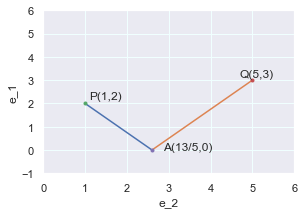
\includegraphics[width=\columnwidth]{./solutions/line_plane/59/output.png}
\caption{Incident and reflected ray vectors plotted via Python code}
\label{fig:solutions/line_plane/59/output1}
\end{figure}
